% L13a figure: a client and a server talk over the Internet.
%
% A desktop computer (the client) sends a request across the Internet cloud to a
% tower computer (the server), and the server sends back a response. The figure
% opens the lecture's Web Services and APIs section.
%
% Drawn on November 13, 2026 with the palette and build of the other L13a
% figures. The notebook SVG carries a dark palette added by theme_svg.py; keep
% new colors in that script's mapping when changing the palette here.
\documentclass[tikz,border=4pt]{standalone}
\usepackage[no-math]{fontspec}
\IfFontExistsTF{Arial}{\setsansfont{Arial}}{\setsansfont{TeX Gyre Heros}}
\IfFontExistsTF{Menlo}{\setmonofont{Menlo}}{}
\renewcommand{\familydefault}{\sfdefault}
\usetikzlibrary{arrows.meta, calc, shapes.symbols}

% Ink, blue, gray, and band match the other L13a figures. Blue marks the request.
% Beige, key, screen, and phosphor draw the two computers.
\definecolor{vnink}{HTML}{202124}
\definecolor{gdblue}{HTML}{0091FF}
\definecolor{gdgray}{HTML}{6D7278}
\definecolor{waband}{HTML}{EEF0F2}
\definecolor{pcbeige}{HTML}{E6DFC8}
\definecolor{pckey}{HTML}{CFC6AA}
\definecolor{crt}{HTML}{23302A}
\definecolor{phosphor}{HTML}{36C26A}

\begin{document}
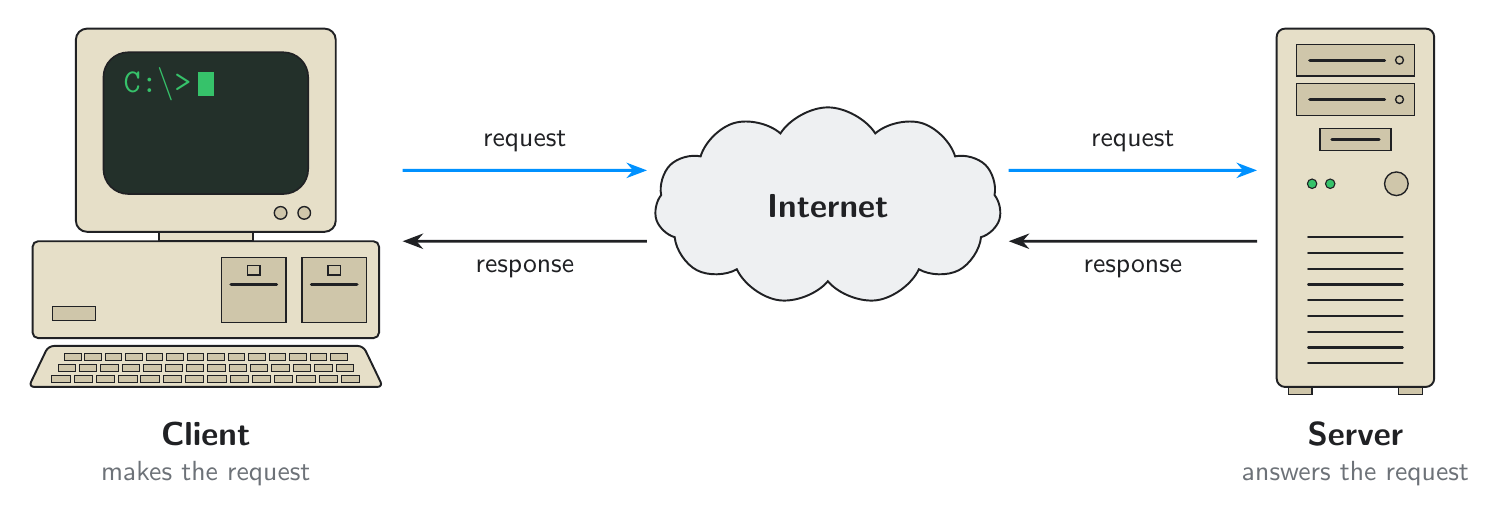
\begin{tikzpicture}[
  font=\sffamily\large,
  >={Stealth[length=2.6mm]},
  case/.style={draw=vnink, fill=pcbeige, line width=0.7pt},
  part/.style={draw=vnink, fill=pckey, line width=0.5pt},
  slot/.style={draw=vnink, line width=1.1pt, line cap=round},
  title/.style={font=\sffamily\large\bfseries, text=vnink},
  note/.style={font=\sffamily\normalsize, text=gdgray, align=center},
  msg/.style={font=\sffamily\normalsize, text=vnink},
  request/.style={->, line width=1.0pt, draw=gdblue},
  response/.style={->, line width=1.0pt, draw=vnink}
]

% ------------------------------------------------- the client: a desktop computer
\begin{scope}[shift={(0, 0)}]
  % keyboard, drawn as a slab that widens toward the viewer
  \draw[case, rounded corners=2pt] (-2.00,-0.98) -- (2.00,-0.98) -- (2.25,-1.50)
    -- (-2.25,-1.50) -- cycle;
  \foreach \r in {0, 1, 2} {
    \pgfmathsetmacro{\half}{1.82 + 0.08*\r}
    \pgfmathsetmacro{\ytop}{-1.07 - 0.14*\r}
    \pgfmathsetmacro{\keyw}{2*\half/14}
    \foreach \k in {0, ..., 13} {
      \draw[part, line width=0.35pt] (-\half + \k*\keyw + 0.025, \ytop)
        rectangle ++(\keyw - 0.05, -0.10);
    }
  }

  % system unit with two floppy drives on the right
  \draw[case, rounded corners=2pt] (-2.20,-0.88) rectangle (2.20,0.35);
  \foreach \x in {0.20, 1.22} {
    \draw[part] (\x,-0.68) rectangle ++(0.82, 0.82);
    \draw[slot] (\x+0.12,-0.20) -- ++(0.58, 0);
    \draw[part] (\x+0.33,-0.08) rectangle ++(0.16, 0.12);
  }
  \draw[part] (-1.95,-0.66) rectangle (-1.40,-0.48);

  % monitor on a short stand, with a dark screen and a prompt
  \draw[case] (-0.60,0.35) rectangle (0.60,0.47);
  \draw[case, rounded corners=4pt] (-1.65,0.47) rectangle (1.65,3.05);
  \draw[draw=vnink, fill=crt, line width=0.6pt, rounded corners=9pt]
    (-1.30,0.95) rectangle (1.30,2.75);
  \node[anchor=west, text=phosphor, font=\ttfamily\large, inner sep=0pt]
    (prompt) at (-1.05,2.35) {C:\textbackslash>};
  \fill[phosphor] ($(prompt.east)+(0.08,-0.15)$) rectangle ++(0.20, 0.30);
  \draw[part] (0.95,0.71) circle (0.08);
  \draw[part] (1.25,0.71) circle (0.08);
\end{scope}

% ------------------------------------------------------------ the Internet
\node[cloud, cloud puffs=11, cloud puff arc=115, aspect=2.1, minimum width=4.4cm,
  minimum height=2.5cm, draw=vnink, fill=waband, line width=0.7pt, title]
  (net) at (7.9, 0.80) {Internet};

% ---------------------------------------------------- the server: a tower computer
\begin{scope}[shift={(14.6, 0)}]
  \draw[part] (-0.85,-1.60) rectangle (-0.55,-1.50);
  \draw[part] (0.55,-1.60) rectangle (0.85,-1.50);
  \draw[case, rounded corners=3pt] (-1.00,-1.50) rectangle (1.00,3.05);

  % two drive bays and a floppy drive
  \foreach \y in {2.45, 1.95} {
    \draw[part] (-0.75,\y) rectangle ++(1.50, 0.40);
    \draw[slot] (-0.58,\y+0.20) -- ++(0.95, 0);
    \draw[part] (0.56,\y+0.20) circle (0.05);
  }
  \draw[part] (-0.45,1.50) rectangle (0.45,1.78);
  \draw[slot] (-0.30,1.64) -- (0.30,1.64);

  % status lights and the power button
  \draw[draw=vnink, fill=phosphor, line width=0.4pt] (-0.55,1.08) circle (0.06);
  \draw[draw=vnink, fill=phosphor, line width=0.4pt] (-0.32,1.08) circle (0.06);
  \draw[part] (0.52,1.08) circle (0.15);

  % air vents
  \foreach \y in {-1.20, -1.00, ..., 0.45} {
    \draw[draw=vnink, line width=0.8pt, line cap=round] (-0.60,\y) -- (0.60,\y);
  }
\end{scope}

% --------------------------------------------- request and response arrows
\draw[request]  (2.50, 1.25) -- ($(net.west)+(-0.10, 0.45)$)
  node[msg, midway, above=3pt] {request};
\draw[response] ($(net.west)+(-0.10,-0.45)$) -- (2.50, 0.35)
  node[msg, midway, below=3pt] {response};
\draw[request]  ($(net.east)+(0.10, 0.45)$) -- (13.35, 1.25)
  node[msg, midway, above=3pt] {request};
\draw[response] (13.35, 0.35) -- ($(net.east)+(0.10,-0.45)$)
  node[msg, midway, below=3pt] {response};

% ------------------------------------------------------------- the labels
\node[title] at (0.0,-2.10)  {Client};
\node[note]  at (0.0,-2.60)  {makes the request};
\node[title] at (14.6,-2.10) {Server};
\node[note]  at (14.6,-2.60) {answers the request};

\end{tikzpicture}
\end{document}
